% Created by tikzDevice version 0.12.6 on 2026-10-29 12:51:06
% !TEX encoding = UTF-8 Unicode
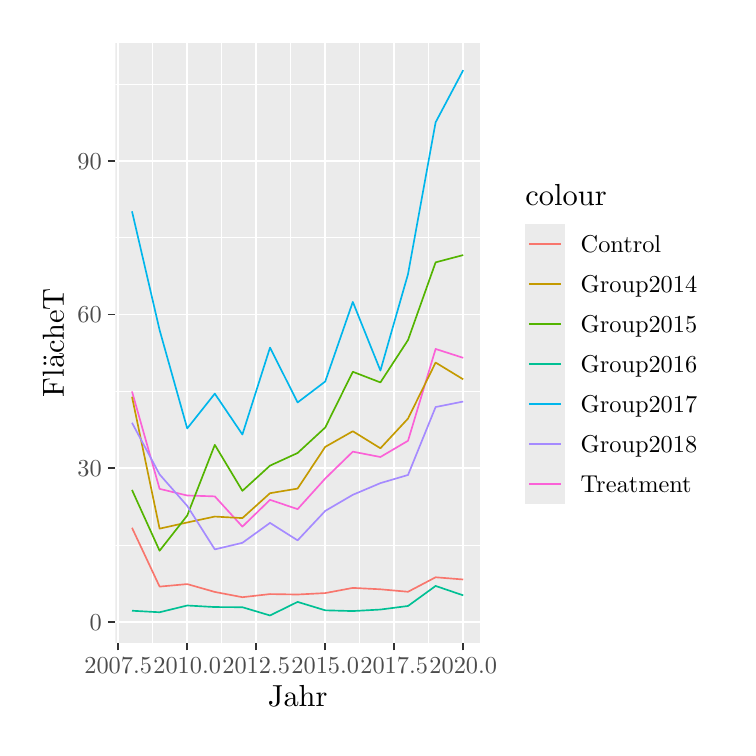
\begin{tikzpicture}[x=1pt,y=1pt]
\definecolor{fillColor}{RGB}{255,255,255}
\path[use as bounding box,fill=fillColor,fill opacity=0.00] (0,0) rectangle (252.94,252.94);
\begin{scope}
\path[clip] (  0.00,  0.00) rectangle (252.94,252.94);
\definecolor{drawColor}{RGB}{255,255,255}
\definecolor{fillColor}{RGB}{255,255,255}

\path[draw=drawColor,line width= 0.6pt,line join=round,line cap=round,fill=fillColor] (  0.00,  0.00) rectangle (252.94,252.94);
\end{scope}
\begin{scope}
\path[clip] ( 31.71, 30.69) rectangle (163.37,247.45);
\definecolor{fillColor}{gray}{0.92}

\path[fill=fillColor] ( 31.71, 30.69) rectangle (163.37,247.45);
\definecolor{drawColor}{RGB}{255,255,255}

\path[draw=drawColor,line width= 0.3pt,line join=round] ( 31.71, 66.00) --
	(163.37, 66.00);

\path[draw=drawColor,line width= 0.3pt,line join=round] ( 31.71,121.51) --
	(163.37,121.51);

\path[draw=drawColor,line width= 0.3pt,line join=round] ( 31.71,177.03) --
	(163.37,177.03);

\path[draw=drawColor,line width= 0.3pt,line join=round] ( 31.71,232.54) --
	(163.37,232.54);

\path[draw=drawColor,line width= 0.3pt,line join=round] ( 45.18, 30.69) --
	( 45.18,247.45);

\path[draw=drawColor,line width= 0.3pt,line join=round] ( 70.11, 30.69) --
	( 70.11,247.45);

\path[draw=drawColor,line width= 0.3pt,line join=round] ( 95.05, 30.69) --
	( 95.05,247.45);

\path[draw=drawColor,line width= 0.3pt,line join=round] (119.98, 30.69) --
	(119.98,247.45);

\path[draw=drawColor,line width= 0.3pt,line join=round] (144.92, 30.69) --
	(144.92,247.45);

\path[draw=drawColor,line width= 0.6pt,line join=round] ( 31.71, 38.25) --
	(163.37, 38.25);

\path[draw=drawColor,line width= 0.6pt,line join=round] ( 31.71, 93.76) --
	(163.37, 93.76);

\path[draw=drawColor,line width= 0.6pt,line join=round] ( 31.71,149.27) --
	(163.37,149.27);

\path[draw=drawColor,line width= 0.6pt,line join=round] ( 31.71,204.78) --
	(163.37,204.78);

\path[draw=drawColor,line width= 0.6pt,line join=round] ( 32.71, 30.69) --
	( 32.71,247.45);

\path[draw=drawColor,line width= 0.6pt,line join=round] ( 57.65, 30.69) --
	( 57.65,247.45);

\path[draw=drawColor,line width= 0.6pt,line join=round] ( 82.58, 30.69) --
	( 82.58,247.45);

\path[draw=drawColor,line width= 0.6pt,line join=round] (107.52, 30.69) --
	(107.52,247.45);

\path[draw=drawColor,line width= 0.6pt,line join=round] (132.45, 30.69) --
	(132.45,247.45);

\path[draw=drawColor,line width= 0.6pt,line join=round] (157.39, 30.69) --
	(157.39,247.45);
\definecolor{drawColor}{RGB}{251,97,215}

\path[draw=drawColor,line width= 0.6pt,line join=round] ( 37.70,121.47) --
	( 47.67, 86.29) --
	( 57.65, 83.89) --
	( 67.62, 83.57) --
	( 77.59, 72.64) --
	( 87.57, 82.33) --
	( 97.54, 78.96) --
	(107.52, 90.02) --
	(117.49, 99.73) --
	(127.46, 97.80) --
	(137.44,103.67) --
	(147.41,136.84) --
	(157.39,133.63);
\definecolor{drawColor}{RGB}{248,118,109}

\path[draw=drawColor,line width= 0.6pt,line join=round] ( 37.70, 72.22) --
	( 47.67, 50.97) --
	( 57.65, 51.88) --
	( 67.62, 49.04) --
	( 77.59, 47.14) --
	( 87.57, 48.27) --
	( 97.54, 48.11) --
	(107.52, 48.63) --
	(117.49, 50.50) --
	(127.46, 50.00) --
	(137.44, 49.10) --
	(147.41, 54.34) --
	(157.39, 53.54);
\definecolor{drawColor}{RGB}{196,154,0}

\path[draw=drawColor,line width= 0.6pt,line join=round] ( 37.70,119.55) --
	( 47.67, 71.91) --
	( 57.65, 74.14) --
	( 67.62, 76.28) --
	( 77.59, 75.72) --
	( 87.57, 84.72) --
	( 97.54, 86.39) --
	(107.52,101.46) --
	(117.49,107.11) --
	(127.46,100.95) --
	(137.44,111.69) --
	(147.41,131.93) --
	(157.39,125.86);
\definecolor{drawColor}{RGB}{83,180,0}

\path[draw=drawColor,line width= 0.6pt,line join=round] ( 37.70, 85.89) --
	( 47.67, 63.93) --
	( 57.65, 76.65) --
	( 67.62,102.19) --
	( 77.59, 85.57) --
	( 87.57, 94.68) --
	( 97.54, 99.25) --
	(107.52,108.46) --
	(117.49,128.60) --
	(127.46,124.75) --
	(137.44,140.07) --
	(147.41,168.14) --
	(157.39,170.77);
\definecolor{drawColor}{RGB}{0,192,148}

\path[draw=drawColor,line width= 0.6pt,line join=round] ( 37.70, 42.25) --
	( 47.67, 41.70) --
	( 57.65, 44.14) --
	( 67.62, 43.58) --
	( 77.59, 43.52) --
	( 87.57, 40.54) --
	( 97.54, 45.44) --
	(107.52, 42.40) --
	(117.49, 42.13) --
	(127.46, 42.68) --
	(137.44, 43.97) --
	(147.41, 51.21) --
	(157.39, 47.80);
\definecolor{drawColor}{RGB}{0,182,235}

\path[draw=drawColor,line width= 0.6pt,line join=round] ( 37.70,186.57) --
	( 47.67,143.68) --
	( 57.65,108.12) --
	( 67.62,120.69) --
	( 77.59,105.94) --
	( 87.57,137.34) --
	( 97.54,117.51) --
	(107.52,125.08) --
	(117.49,153.84) --
	(127.46,129.03) --
	(137.44,163.91) --
	(147.41,218.74) --
	(157.39,237.59);
\definecolor{drawColor}{RGB}{165,138,255}

\path[draw=drawColor,line width= 0.6pt,line join=round] ( 37.70,110.16) --
	( 47.67, 91.51) --
	( 57.65, 80.14) --
	( 67.62, 64.42) --
	( 77.59, 66.79) --
	( 87.57, 73.99) --
	( 97.54, 67.68) --
	(107.52, 78.32) --
	(117.49, 84.14) --
	(127.46, 88.36) --
	(137.44, 91.31) --
	(147.41,115.86) --
	(157.39,117.84);
\end{scope}
\begin{scope}
\path[clip] (  0.00,  0.00) rectangle (252.94,252.94);
\definecolor{drawColor}{gray}{0.30}

\node[text=drawColor,anchor=base east,inner sep=0pt, outer sep=0pt, scale=  0.88] at ( 26.76, 35.22) {0};

\node[text=drawColor,anchor=base east,inner sep=0pt, outer sep=0pt, scale=  0.88] at ( 26.76, 90.73) {30};

\node[text=drawColor,anchor=base east,inner sep=0pt, outer sep=0pt, scale=  0.88] at ( 26.76,146.24) {60};

\node[text=drawColor,anchor=base east,inner sep=0pt, outer sep=0pt, scale=  0.88] at ( 26.76,201.75) {90};
\end{scope}
\begin{scope}
\path[clip] (  0.00,  0.00) rectangle (252.94,252.94);
\definecolor{drawColor}{gray}{0.20}

\path[draw=drawColor,line width= 0.6pt,line join=round] ( 28.96, 38.25) --
	( 31.71, 38.25);

\path[draw=drawColor,line width= 0.6pt,line join=round] ( 28.96, 93.76) --
	( 31.71, 93.76);

\path[draw=drawColor,line width= 0.6pt,line join=round] ( 28.96,149.27) --
	( 31.71,149.27);

\path[draw=drawColor,line width= 0.6pt,line join=round] ( 28.96,204.78) --
	( 31.71,204.78);
\end{scope}
\begin{scope}
\path[clip] (  0.00,  0.00) rectangle (252.94,252.94);
\definecolor{drawColor}{gray}{0.20}

\path[draw=drawColor,line width= 0.6pt,line join=round] ( 32.71, 27.94) --
	( 32.71, 30.69);

\path[draw=drawColor,line width= 0.6pt,line join=round] ( 57.65, 27.94) --
	( 57.65, 30.69);

\path[draw=drawColor,line width= 0.6pt,line join=round] ( 82.58, 27.94) --
	( 82.58, 30.69);

\path[draw=drawColor,line width= 0.6pt,line join=round] (107.52, 27.94) --
	(107.52, 30.69);

\path[draw=drawColor,line width= 0.6pt,line join=round] (132.45, 27.94) --
	(132.45, 30.69);

\path[draw=drawColor,line width= 0.6pt,line join=round] (157.39, 27.94) --
	(157.39, 30.69);
\end{scope}
\begin{scope}
\path[clip] (  0.00,  0.00) rectangle (252.94,252.94);
\definecolor{drawColor}{gray}{0.30}

\node[text=drawColor,anchor=base,inner sep=0pt, outer sep=0pt, scale=  0.88] at ( 32.71, 19.68) {2007.5};

\node[text=drawColor,anchor=base,inner sep=0pt, outer sep=0pt, scale=  0.88] at ( 57.65, 19.68) {2010.0};

\node[text=drawColor,anchor=base,inner sep=0pt, outer sep=0pt, scale=  0.88] at ( 82.58, 19.68) {2012.5};

\node[text=drawColor,anchor=base,inner sep=0pt, outer sep=0pt, scale=  0.88] at (107.52, 19.68) {2015.0};

\node[text=drawColor,anchor=base,inner sep=0pt, outer sep=0pt, scale=  0.88] at (132.45, 19.68) {2017.5};

\node[text=drawColor,anchor=base,inner sep=0pt, outer sep=0pt, scale=  0.88] at (157.39, 19.68) {2020.0};
\end{scope}
\begin{scope}
\path[clip] (  0.00,  0.00) rectangle (252.94,252.94);
\definecolor{drawColor}{RGB}{0,0,0}

\node[text=drawColor,anchor=base,inner sep=0pt, outer sep=0pt, scale=  1.10] at ( 97.54,  7.64) {Jahr};
\end{scope}
\begin{scope}
\path[clip] (  0.00,  0.00) rectangle (252.94,252.94);
\definecolor{drawColor}{RGB}{0,0,0}

\node[text=drawColor,rotate= 90.00,anchor=base,inner sep=0pt, outer sep=0pt, scale=  1.10] at ( 13.08,139.07) {FlächeT};
\end{scope}
\begin{scope}
\path[clip] (  0.00,  0.00) rectangle (252.94,252.94);
\definecolor{fillColor}{RGB}{255,255,255}

\path[fill=fillColor] (174.37, 75.37) rectangle (247.44,202.76);
\end{scope}
\begin{scope}
\path[clip] (  0.00,  0.00) rectangle (252.94,252.94);
\definecolor{drawColor}{RGB}{0,0,0}

\node[text=drawColor,anchor=base west,inner sep=0pt, outer sep=0pt, scale=  1.10] at (179.87,188.62) {colour};
\end{scope}
\begin{scope}
\path[clip] (  0.00,  0.00) rectangle (252.94,252.94);
\definecolor{fillColor}{gray}{0.92}

\path[fill=fillColor] (179.87,167.59) rectangle (194.33,182.05);
\definecolor{drawColor}{RGB}{248,118,109}

\path[draw=drawColor,line width= 0.6pt,line join=round] (181.32,174.82) -- (192.88,174.82);
\end{scope}
\begin{scope}
\path[clip] (  0.00,  0.00) rectangle (252.94,252.94);
\definecolor{fillColor}{gray}{0.92}

\path[fill=fillColor] (179.87,153.14) rectangle (194.33,167.59);
\definecolor{drawColor}{RGB}{196,154,0}

\path[draw=drawColor,line width= 0.6pt,line join=round] (181.32,160.37) -- (192.88,160.37);
\end{scope}
\begin{scope}
\path[clip] (  0.00,  0.00) rectangle (252.94,252.94);
\definecolor{fillColor}{gray}{0.92}

\path[fill=fillColor] (179.87,138.69) rectangle (194.33,153.14);
\definecolor{drawColor}{RGB}{83,180,0}

\path[draw=drawColor,line width= 0.6pt,line join=round] (181.32,145.91) -- (192.88,145.91);
\end{scope}
\begin{scope}
\path[clip] (  0.00,  0.00) rectangle (252.94,252.94);
\definecolor{fillColor}{gray}{0.92}

\path[fill=fillColor] (179.87,124.23) rectangle (194.33,138.69);
\definecolor{drawColor}{RGB}{0,192,148}

\path[draw=drawColor,line width= 0.6pt,line join=round] (181.32,131.46) -- (192.88,131.46);
\end{scope}
\begin{scope}
\path[clip] (  0.00,  0.00) rectangle (252.94,252.94);
\definecolor{fillColor}{gray}{0.92}

\path[fill=fillColor] (179.87,109.78) rectangle (194.33,124.23);
\definecolor{drawColor}{RGB}{0,182,235}

\path[draw=drawColor,line width= 0.6pt,line join=round] (181.32,117.00) -- (192.88,117.00);
\end{scope}
\begin{scope}
\path[clip] (  0.00,  0.00) rectangle (252.94,252.94);
\definecolor{fillColor}{gray}{0.92}

\path[fill=fillColor] (179.87, 95.32) rectangle (194.33,109.78);
\definecolor{drawColor}{RGB}{165,138,255}

\path[draw=drawColor,line width= 0.6pt,line join=round] (181.32,102.55) -- (192.88,102.55);
\end{scope}
\begin{scope}
\path[clip] (  0.00,  0.00) rectangle (252.94,252.94);
\definecolor{fillColor}{gray}{0.92}

\path[fill=fillColor] (179.87, 80.87) rectangle (194.33, 95.32);
\definecolor{drawColor}{RGB}{251,97,215}

\path[draw=drawColor,line width= 0.6pt,line join=round] (181.32, 88.10) -- (192.88, 88.10);
\end{scope}
\begin{scope}
\path[clip] (  0.00,  0.00) rectangle (252.94,252.94);
\definecolor{drawColor}{RGB}{0,0,0}

\node[text=drawColor,anchor=base west,inner sep=0pt, outer sep=0pt, scale=  0.88] at (199.83,171.79) {Control};
\end{scope}
\begin{scope}
\path[clip] (  0.00,  0.00) rectangle (252.94,252.94);
\definecolor{drawColor}{RGB}{0,0,0}

\node[text=drawColor,anchor=base west,inner sep=0pt, outer sep=0pt, scale=  0.88] at (199.83,157.34) {Group2014};
\end{scope}
\begin{scope}
\path[clip] (  0.00,  0.00) rectangle (252.94,252.94);
\definecolor{drawColor}{RGB}{0,0,0}

\node[text=drawColor,anchor=base west,inner sep=0pt, outer sep=0pt, scale=  0.88] at (199.83,142.88) {Group2015};
\end{scope}
\begin{scope}
\path[clip] (  0.00,  0.00) rectangle (252.94,252.94);
\definecolor{drawColor}{RGB}{0,0,0}

\node[text=drawColor,anchor=base west,inner sep=0pt, outer sep=0pt, scale=  0.88] at (199.83,128.43) {Group2016};
\end{scope}
\begin{scope}
\path[clip] (  0.00,  0.00) rectangle (252.94,252.94);
\definecolor{drawColor}{RGB}{0,0,0}

\node[text=drawColor,anchor=base west,inner sep=0pt, outer sep=0pt, scale=  0.88] at (199.83,113.97) {Group2017};
\end{scope}
\begin{scope}
\path[clip] (  0.00,  0.00) rectangle (252.94,252.94);
\definecolor{drawColor}{RGB}{0,0,0}

\node[text=drawColor,anchor=base west,inner sep=0pt, outer sep=0pt, scale=  0.88] at (199.83, 99.52) {Group2018};
\end{scope}
\begin{scope}
\path[clip] (  0.00,  0.00) rectangle (252.94,252.94);
\definecolor{drawColor}{RGB}{0,0,0}

\node[text=drawColor,anchor=base west,inner sep=0pt, outer sep=0pt, scale=  0.88] at (199.83, 85.07) {Treatment};
\end{scope}
\end{tikzpicture}
